
\part{Appendix}

%\setcounter{chapter}{1}
%\renewcommand{\thechapter}{\Roman{chapter}}
%\renewcommand{\thesection}{\Roman{chapter}.\arabic{section}}

\appendix

\chapter{ITI Project}
\label{ch:itiProject}

\begin{wrapfigure}{r}{60mm}
  \vspace{-5cm}
  
\includegraphics[width=60mm]{part4/pics/itiLogo.png}
  \vspace{-5cm}
\end{wrapfigure}

The ITI(Intuitive Touch-screen Interface) project was a collaborative project involving the INRIA, and the LOUSTIC laboratory, in the global context of the IDA project. The LOUSTIC\footnote{http://www.loustic.net/} is a laboratory of observation of the use of Information and Communication Technologies(ICT), which measures people reactions with relation to a given technology. Tests of artefacts are realized by volunteers, belonging to a pre-defined part of the population. According to the product under test, several measurements can be performed such as time spent to find an information, eye-tracking, reactivity of the product, etc.\\

\enti{} is designed to allow dynamic and unpredicted changes in terms of components or services. Any end-user oriented control interface for an EnTiMid running system have to be able to deal with these changes at runtime. In this context, the creation of a universal Graphical User Interface(GUI) sounds like a complicated task. To cope with this problem, the idea of an automatic generation of \gls{gui} has been proposed. From this perspective, devices have been imagined able to provide an abstract description of the graphical controls they require.\\
In addition, \gls{gui} can be constraint by users' preferences, or needs in terms of font size for a an elderly person, or a nurse. The idea is to adapt the graphical user interface during the execution. Some work, presented in\cite{Blouin:2011}, has already been engaged in this way.\\

If the automatic generation of \gls{gui} appeared as a really interesting field of research, the amount of work to achieve a first proof of concept appeared to be huge. Therefore, it has been decided to first sketch an application GUI, adapted to elderly people, before actually performing the generative work. The sketch of this GUI, and the measurement of its usability by elderly people was the goal of the ITI project. It also validates that the GUI of this contribution is acceptable, and accessible, for elderly people, which are part of requirements listed in section~\ref{ch:requirements}.\\

The results presented in this chapter have been extracted from the internship report~\cite{COLAS:2009} of E. Colas and N. Courtais, who actually realised the tests.

\section{Presentation and Goals of the project}

In the \gls{aal} context, people must be able to interact with the assisting system. Since a great part of the end-users in this context are elderly people, the control interface of any solution built with \enti{} must be adapted. The adaptation of an interface to the elderly population obviously concerns some ergonomic aspects. However, the visual aspect was treated as a secondary goal. The main concern was about the navigation method to be implemented. In the domain of home automation control interface, two methods of navigation can be applied. The first consists in selecting the location first, then the function to be considered. On the other hand, the function is selected first and the zone concerned after. Thus, the leading question of the project was: Is it more convenient for people to navigate by Zone then Function, or by Function then Zone ?\\
To answer this question, and design a relevant GUI sketch, the project had been split into three phases.\\

\subsection{Phase 1}
This phase did consist in designing the graphical interface, according to well know ergonomics rules~\cite{Bastien:1993}. In this phase, attention was paid to the size of each element (buttons, text, labels, etc.), for them to be easily readable, and for the information not to be lost in useless decorative elements. At the end of this phase, two graphical interfaces were released. The first was implementing the Function/Zone navigation mode; the second, the Zone/Function one.\\
Figure~\ref{fig:phaseOneInterfaces} presents the graphical user interfaces created in this phase. Three screenshot of the Function/Zone proposition are visible on the first line of the figure, while the bottom left screenshot displays one of the three Zone/Function screen. All the widgets used are shown on the bottom right part of the figure.

\begin{figure}[h!]
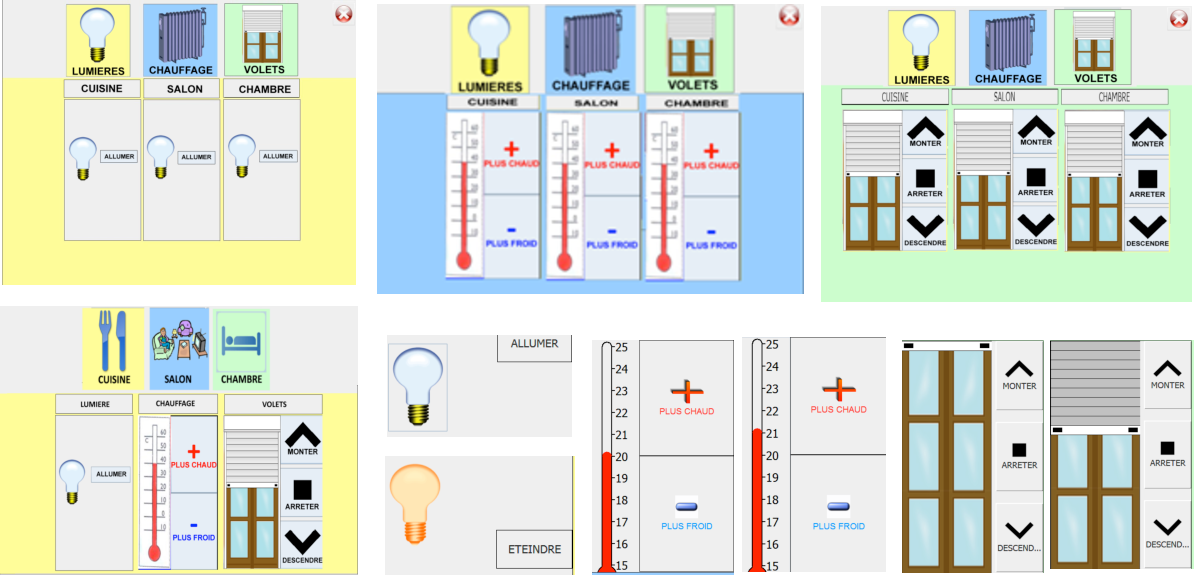
\includegraphics[width=\textwidth]{part4/pics/PhaseOneInterfaces}
\caption{Results of the first phase}
\label{fig:phaseOneInterfaces}
\end{figure}


\subsection{Phase 2}
Phase 2 aimed at presenting the interfaces to elderly people. Measures have been realized on their first reactions with relation to the navigation mode they preferred, and on their ability to use the controls and retrieve information from the system. The second phase improved the graphical interfaces in terms of controls, and information presentation, for these elements to be of minimum influence on the answers to the navigation question.\\
The main improvements concerned the widgets themselves. The light widget has been reduced to a single light bulb, which aspect clearly indicates the state of the light, and a touch of the bulb toggle the state of the light. This improvement is visible at the bottom of figure~\ref{fig:phaseTwoInterfaces}. No change has been made on shutter widgets, but the temperature widget was simplified, by the removal of the plus and minus buttons, since elderly people just pressed on the thermometer.\\
The figure only shows Function/Zone interfaces, but the modifications on widgets have also been realized on the Zone/Function interface the same way.

\begin{figure}[h!]
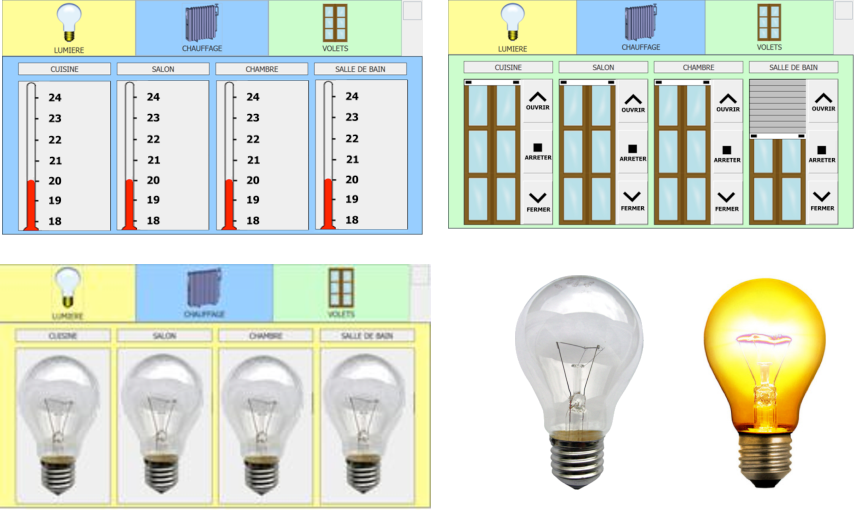
\includegraphics[width=\textwidth]{part4/pics/PhaseTwoInterfaces}
\caption{Improved interfaces, result of the second phase}
\label{fig:phaseTwoInterfaces}
\end{figure}

\subsection{Phase 3}
This last phase resumed the tests with elderly people, using the improved user interfaces. 

\section{Environment of tests}

\subsection{Population under test}
Altogether, 20 persons from 72 to 97 years old, with a median age of 82 years old, participated to the test within four groups. The tests were realized in two different care centres for elderly people, during their activity time.\\

\subsection{Equipments}
\begin{itemize}
\item The main equipment was a MSI Top "all-in-one" touch-screen PC, on which the two interfaces had been deployed.
\item For measurement concerns, the "CamStudio" software was installed on the PC to record the actions of the user on the \gls{gui}, and a camera filmed the activity of the person.
\item A slideshow, made of three slides, was used to present the touch-screen pc, and how to use it.
\item Several questionnaires were set up to collect different information, and guide the tests: personal information(age, sex, school level, etc.), skills and fears with relation to computers, seven scenarios to measure interfaces, and a last questionnaire about how they felt during the test, and how they perceived \enti{} and its interfaces. These questionnaires, in French, are available in the report~\cite{COLAS:2009}.

\end{itemize}


\section{Protocol of test}
\begin{enumerate}
\item First of all, people are asked to answer the first questionnaire about personal information, and the one about their skills and fears.
\item Once the first questionnaires is answered, the slideshow is played in interaction with the elderly person. Guided by the test driver, the person has to move forward the slides, by pressing a button on the touch-screen, in order for the person to familiarize with this technology.
\item The next step is a short training on the user interface under test. In a couple of minutes, the test driver presents the different controls, how to use them, what they can be used for, and where to find important information such as the current location.
\item The real test phase of the protocol is then engaged. The person is asked to realize a sequence of seven actions. These actions ask whether to act on the interface, or to get an information from the system.
\item The questionnaire about their feelings, and the use of these interfaces, is filled at the end of each test.

\end{enumerate}

\section{Threats to validity}

The study had been led with only 20 elderly people. It is not sufficient to validate the \gls{gui} for a large-scale deployment, but it is for a preliminary work.\\
Moreover, the part of the population targeted by the IDA project is considered to be able to stay at home with a little help. These persons are thus living at home, and not in a care centre for elderly people. The conditions in which this study was led can thus be considered as too strict with relation to the real part of population targeted by the project.

\section{Results and conclusion}

The table~\ref{table:efficiencyInterafces} presents the results of the tests. The time values displayed are all in seconds, and represent the average values of execution of each task. The total execution time column reports the average time necessary for people to complete the seven tasks of questionnaire. The other columns are the average time of execution, used to answer the particular questions of the questionnaire for each widget.

\begin{table}[h!]
\centering
\begin{tabular}{|c|c|>{\centering\arraybackslash}m{.12\textwidth}|>{\centering\arraybackslash}m{.12\textwidth}|>{\centering\arraybackslash}m{.12\textwidth}|>{\centering\arraybackslash}m{.12\textwidth}|}
\cline{3-6}
 \multicolumn{2}{c|}{ } &  Total Execution Time(s) & Heating Widget & Shutter Widget & Light Widget\\
\hline
\multirow{2}{*}{Function/Zone}
 & Phase 1 & {\centering 620},83 & 96 & 35,3 & 12,3 \\
 & Phase 2 & 238,75 & 14,25 & 16,75 & 6,25\\
\hline
\multirow{2}{*}{Zone/Function} 
 & Phase 1 & 697 & 74 & 44,5 & 8\\
 & Phase 2 & 429,6 & 37,4 & 36,8 & 8\\
 \hline
\end{tabular}
\caption{Efficiency of use with relation to interfaces types}
\label{table:efficiencyInterafces}
\end{table}

{\bf Significant improvement from Phase 1 to Phase 2}\\
The total average execution time has been reduced of 62\% in the Function/Zone mode, and 38\% in the other mode, simply because of the improvement of the widgets.\\

{\bf Function/Zone better than Zone/Function ?}\\
The answer is YES. The Function/Zone navigation mode is more efficient than the Zone/Function mode. Whatever the phase of the project, people have always been faster using the Function/Zone mode, according to the data collected. This can be due to the radical change that occurs when passing from a function to another, which is not the case when changing of zone. Indeed, in each zone the widgets are the same, and only a label changes. All the widgets are changing from a function to another, making it easier to understand what is the current function, and then, identify where to activate this function.\\

I would like to highlight the huge difference in execution time, between the Phase 1 - Zone/Function interface, and the Phase 2 - Function/Zone interface. It is a gain of 458,25 seconds, thus 7 minutes 38 seconds.\\
As a conclusion, the ITI project helped in validating three things. (1) It is more efficient to use a Function/Zone navigation than a Zone/Function. (2) The widgets are now ready. (3) The sketched application \gls{gui} can be used by elderly people on a touch-screen device, which answers the accessibility and usability requirement.

